\documentclass[10pt,a4paper]{article}
\usepackage{amsmath,amssymb,amsthm,graphicx}
\usepackage{amsmath,amssymb,mathtools}
\usepackage{hyperref}
\usepackage{graphicx}
\usepackage{fontspec}
\setmainfont{DejaVu Serif}
\sloppy
\setlength{\emergencystretch}{3em}
\title{Optimal deterministic trapezoidal decomposition of disjoint polygonal chains and triangulation with holes}
\author{Timothy M. Chan}
\date{doi:10.4230/LIPIcs.SoCG.2026.28; CC BY 4.0}
\begin{document}
\maketitle
\noindent\textit{Editorial scope.} Complete official sections 1–3 and References. Count Theorem1 and its immediate polygon-with-holes application together. Intersection extensions of section4/AppendixA are not counted or required. The algorithm combines interval-tree grouping and Jordan sorting with two levels of planar r-division. It builds a deterministic edge subset with vertical-segment intersection control, cuts chains across the second division, and balances s=log\textasciicircum{}2 n and t=log\textasciicircum{}8 n to achieve O(n+h log h). The source-specific construction and complete parameter/time analysis remain in this task.\par\medskip
\noindent\textit{Allowed standard prerequisites (editorial).}\begin{itemize}
\item Classical Chazelle linear-time simple-polygon triangulation; Bar-Yehuda–Chazelle Jordan sorting/chain decomposition algorithms; standard planar r-division and point location.. Exact author external statements are in official sections 1–3, references [3], [5], [16], [18], [21], [26]. These classical algorithms remain cited black boxes; all new source-specific sampling/division and cost arguments are included.
\end{itemize}\medskip
% BEGIN S1
\par\medskip\noindent\textbf{1 Introduction}\par
% BEGIN S1.p1
Triangulating a simple polygon is one of the most basic problems in computational geometry, with numerous applications. Chazelle’s deterministic linear-time algorithm [5] represents one of the landmark results in the area, improving previous deterministic $O(n\log\log n)$-time algorithms by Tarjan and Van Wyck [28] and Kirkpatrick, Klawe, and Tarjan [20] and previous randomized $O(n\log^{*}n)$-time algorithms by Clarkson, Tarjan, and Van Wyck [10] and Seidel [27]. Here, $n$ denotes the number of vertices in the input polygon and $\log^{*}$ is the (very slow-growing) iterated logarithm function.
\par
\par
% END S1.p1
% BEGIN S1.p2
In this paper, we study an extension of the problem: triangulating a polygon with $h$ holes (where the holes themselves are disjoint simple polygons enclosed in an outer simple polygon). See Figure 1 (left). The problem can be equivalently stated in a number of different ways:
\par
\begin{enumerate}
\item[]  1. 
Computing the trapezoidal decomposition of a polygon with $h$ holes. The decomposition (also called the “trapezoidization”, or “vertical decomposition”, or “vertical visibility map”) is obtained by adding vertical line segments from each vertex to the edge immediately above/below the vertex. Linear-time reductions from trapezoidal decompositions to triangulations and vice versa are known [14].
\par
\par
\item[]  2. 
Computing the trapezoidal decomposition of a collection of $h$ disjoint simple polygonal chains. See Figure 1 (right). (We can enclose the chains with a bounding box and turn each chain into an infinitesimally thin hole, while increasing $n$ and $h$ by only a constant factor.)
\par
\par
\item[]  3. 
Computing the trapezoidal decomposition of a plane straight-line graph (a graph drawn on the plane with straight-line edges without crossings, where edges are ordered around each vertex) with $h$ connected components. (We can make tiny cuts to eliminate cycles and then take an Euler tour to turn each component into a chain, while increasing $n$ and $h$ by only a constant factor.)
\par
\par
\end{enumerate}
\par
% END S1.p2
% BEGIN S1.F1
\begin{center}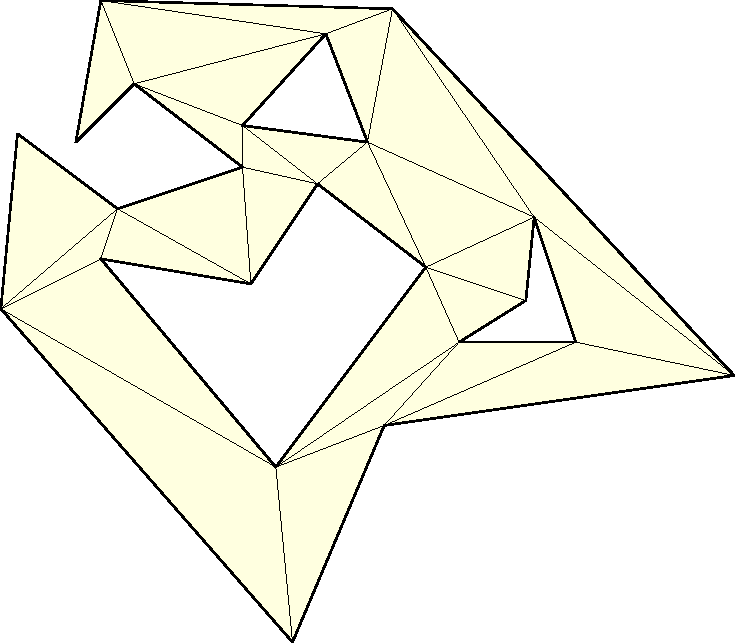
\includegraphics[width=0.7\linewidth,height=0.38\textheight,keepaspectratio]{fig_polygon-page-1.pdf2svg.pdf}\end{center}
\begin{center}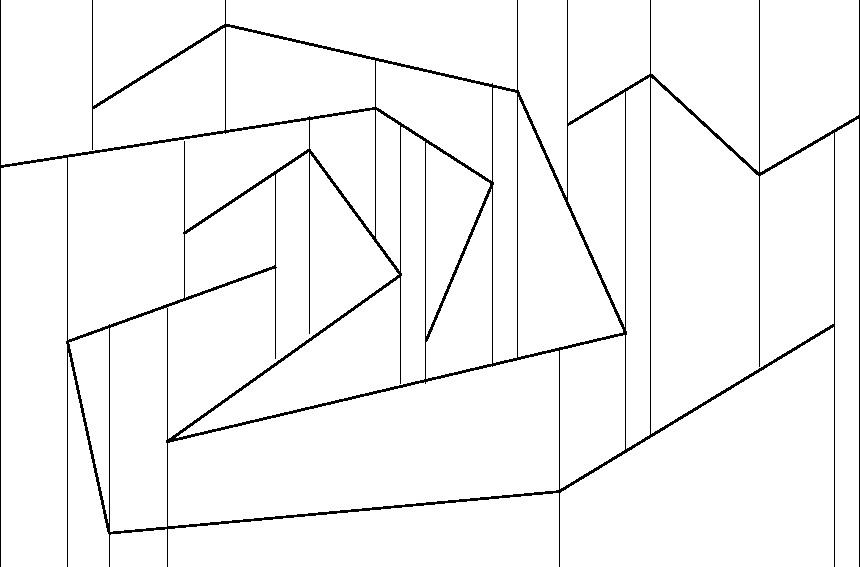
\includegraphics[width=0.7\linewidth,height=0.38\textheight,keepaspectratio]{fig_polygon-page-2.pdf2svg.pdf}\end{center}
  Figure 1: (Left) A triangulation of a polygon with 3 holes. (Right) The trapezoidal decomposition of 5 disjoint simple polygonal chains. 
% END S1.F1
% BEGIN S1.p3
Previous randomized $O(n\log^{*}n)$-time algorithms for simple polygons can be adapted to solve the problem in $O(n\log^{*}n+h\log h)$ expected time [8, 27]. In 1994, Bar-Yehuda and Chazelle [3] gave deterministic algorithms running in $O(\min\{n+h\log^{1+\varepsilon}h,\,(n+h\log h)\log\log h\})$ time for an arbitrarily small constant $\varepsilon>0$. These results came close to the known lower bound of $\Omega(n+h\log h)$,\footnote{An $\Omega(h\log h)$ lower bound in the algebraic decision tree model can be shown by a simple reduction from sorting: to sort $h$ numbers $x_{1},\ldots,x_{h}\in(-1,1)$, create a polygon that has a triangular outer boundary with vertices $(-1,1),(1,1),(0,-1)$, and a sufficiently small hole near $(x_{i},x_{i}^{2})$ for each $i\in\{1,\ldots,h\}$. } but there is still an extra factor of $\log^{*}n$ for randomized algorithms, and $\log^{\varepsilon}h$ or $\log\log h$ for deterministic. No improvement has been reported since, deterministic or randomized.
\par
\par
% END S1.p3
% BEGIN S1.p4
Meanwhile, a number of papers (e.g., [7, 19, 24, 29]) have given algorithms for various problems related to shortest paths and visibility in polygonal domains (polygonal environments with multiple disjoint polygonal obstacles) whose time complexities are dominated by that of the triangulation problem and would be optimal if the triangulation complexity is $O(n+h\log h)$. However, with the current gap of knowledge, these papers needed to state their results more awkwardly, either by assuming that a triangulation of the free space of the polygonal domain (a polygon with holes) is given, or by adding an extra term $T$ to the time bound where $T$ represents the unknown complexity of the triangulation problem. (A similar story occurred for various computational problems about simple polygons in the days before Chazelle’s linear-time algorithm.)
\par
\par
% END S1.p4
% BEGIN S1.SS0.SSS0.P0.SPx1
\par\medskip\noindent\textbf{Main result.}\par
% BEGIN S1.SS0.SSS0.P0.SPx1.p1
We give the first optimal algorithm for triangulating a polygon with holes in $O(n+h\log h)$ time. The algorithm is deterministic.
\par
\par
% END S1.SS0.SSS0.P0.SPx1.p1
% BEGIN S1.SS0.SSS0.P0.SPx1.p2
Many applications follow [7, 19, 24, 29]. (For example, combining with Wang’s result [29] yields an optimal $O(n+h\log h)$-time algorithm for finding the Euclidean shortest path between two given points amidst $h$ disjoint polygonal obstacles with $n$ vertices total.)
\par
\par
% END S1.SS0.SSS0.P0.SPx1.p2
% END S1.SS0.SSS0.P0.SPx1
% BEGIN S1.SS0.SSS0.P0.SPx2
\par\medskip\noindent\textbf{Previous approaches.}\par
% BEGIN S1.SS0.SSS0.P0.SPx2.p1
Known approaches, as well as our new algorithm, work with the reformulation of the problem in terms of the trapezoidal decomposition of $h$ disjoint polygonal chains.
\par
\par
% END S1.SS0.SSS0.P0.SPx2.p1
% BEGIN S1.SS0.SSS0.P0.SPx2.p2
One could try to directly modify Chazelle’s linear-time algorithm for $h=1$ [5], but this appears difficult (considering how notoriously complicated his algorithm was). Bar-Yehuda and Chazelle’s approach was to directly reduce the general $h$ case to the $h=1$ case: join the multiple polygonal chains into one connected component by adding vertical line segments, and then apply Chazelle’s algorithm as a black box. To do so, the first observation is that polygonal chains intersecting a common vertical line can be joined together this way by Jordan sorting (the problem of sorting intersections of polygonal chains along a line), which is solvable by known techniques [18]. Roughly, their idea was then to build an interval tree [11, 26] for the $x$-spans of the chains, and solve the problem for each level of the interval tree (since each level consists of vertically separated instances in which chains intersect a common vertical line). The remaining task is merging the results of these $O(\log h)$ levels. Bar-Yehuda and Chazelle proposed a binary divide-and-conquer over the $O(\log h)$ levels, yielding $O((n+h\log h)\log\log h)$ time overall, and alternatively a divide-and-conquer with a larger fan-out, yielding $O(n+h\log^{1+\varepsilon}h)$. This approach seems hard to improve further.
\par
\par
% END S1.SS0.SSS0.P0.SPx2.p2
% BEGIN S1.SS0.SSS0.P0.SPx2.p3
A different approach is randomized divide-and-conquer, as done by Clarkson et al. and Seidel [10, 27]. The trapezoidal decomposition of a random sample of $n/\log n$ edges allows us to divide the problem into subproblems of roughly logarithmic size. Assigning input elements to subproblems requires some form of “point location” and would normally cost $O(\log n)$ per element, but can be done faster knowing that the input elements comes from $h$ chains. Since the recursion has $O(\log^{*}n)$ levels, the running time inherently increases by a $\log^{*}n$ factor, unfortunately. Even for $h=1$ (the case of a simple polygon), Clarkson et al. and Seidel’s methods do not achieve linear time (Amato, Goodrich, and Ramos [1] described a randomized linear-time algorithm which is simpler than Chazelle’s, but still relies on some of Chazelle’s ingredients and is still complicated). Furthermore, randomization seems essential: such random sampling methods where the sample size is large is generally harder to derandomize.
\par
\par
% END S1.SS0.SSS0.P0.SPx2.p3
% END S1.SS0.SSS0.P0.SPx2
% BEGIN S1.SS0.SSS0.P0.SPx3
\par\medskip\noindent\textbf{Our approach.}\par
% BEGIN S1.SS0.SSS0.P0.SPx3.p1
The difficulty of improving the random sampling approach turns out to be overstated. We observe that in combination with another known divide-and-conquer strategy via planar graph separators [22] or $r$-divisions [15, 16], the random sampling approach can indeed achieve optimal $O(n+h\log h)$ expected running time. The reason the $\log^{*}n$ factor is avoidable is that we can recurse for a constant number of levels (in fact, just once) and then switch to Chazelle’s algorithm (or more precisely Bar-Yehuda and Chazelle’s algorithm, which calls Chazelle’s) in the base case when the input size is sufficiently small – the $h\log h$ term is big enough to absorb the cost of the switch. The idea of combining sampling with $r$-divisions and invoking Chazelle’s in the base case is not original and can be viewed as a variant of an existing randomized algorithm by Eppstein, Goodrich, and Strash [13] for a related problem (see below). Still, it is interesting that this implication has not been noted earlier, and we include this optimal randomized solution in Appendix A.
\par
\par
% END S1.SS0.SSS0.P0.SPx3.p1
% BEGIN S1.SS0.SSS0.P0.SPx3.p2
Our main contribution is in obtaining an optimal deterministic algorithm. To do so, we combine ideas from both the random sampling approach and Bar-Yehuda and Chazelle’s deterministic approach, even though the two approaches appear different and incompatible. To derandomize the sampling approach, we need to compute a subset of the input edges that “behave” like a random sample, known as an $\varepsilon$-net in the literature [17, 23] (with $\varepsilon$ being $\frac{\mathop{\rm polylog}n}{n}$ in our case). Constructing a net deterministically appears challenging, especially since we can only afford linear time. We observe a simple way to construct a net in linear time when the trapezoidal decomposition is given, by using planar graph separators or $r$-divisions (the net size is suboptimal, but is good enough for our purposes).
\par
\par
% END S1.SS0.SSS0.P0.SPx3.p2
% BEGIN S1.SS0.SSS0.P0.SPx3.p3
However, there is an obvious circularity issue: we are not given the trapezoidal decomposition, since that is what we want to compute! Our key idea is to go back to Bar-Yehuda and Chazelle’s interval-tree approach, which gives a partition of the input into $O(\log n)$ subsets where we already know how to compute the trapezoidal decomposition of each subset. Although merging their trapezoidal decompositions is not easy, merging their nets is: the union of the nets of the subsets is a net for the whole input (the net size is worsen by an $O(\log n)$ factor, but is still good enough for our purposes). By building the trapezoidal decomposition of the net in combination with an $r$-division, we can then divide the problem into subproblems of polylogarithmic size. The detailed description of the whole algorithm is given in Section 3, and is just about 2 pages long.
\par
\par
% END S1.SS0.SSS0.P0.SPx3.p3
% END S1.SS0.SSS0.P0.SPx3
% BEGIN S1.SS0.SSS0.P0.SPx4
\par\medskip\noindent\textbf{When there are intersections.}\par
% BEGIN S1.SS0.SSS0.P0.SPx4.p1
In the last part of the paper, we address an extension of the problem: computing the trapezoidal decomposition of polygonal chains that may not be simple, i.e., may self-intersect, and may intersect each other. The decomposition is defined in the same way, except that we also add vertical segments from each intersection point to the edge immediately above/below. The crux of the problem lies in the computation of the intersections. (Once all the intersection points are known, we could actually reduce to the non-intersecting case to obtain the final trapezoidal decomposition.)
\par
\par
% END S1.SS0.SSS0.P0.SPx4.p1
% BEGIN S1.SS0.SSS0.P0.SPx4.p2
The problem of computing all self-intersections of one chain (the $h=1$ case) is already challenging. Chazelle [5] posed the (still open) question of whether there is an $O(n+X)$-time algorithm, where $X$ denotes the number of intersections. Known line-segment intersection algorithms [9, 25, 6, 2] can solve the problem in $O(n\log n+X)$ time, which is optimal when $X\gg n\log n$ but not when $X$ is sublinear; they do not exploit the fact that the input line segments form a connected chain. Clarkson, Cole, Tarjan [8] showed that the random sampling approach yields an $O(n\log^{*}n+X)$ expected time bound for this problem. On the other hand, Eppstein, Goodrich, and Strash [13] used random sampling in combination with $r$-divisions to obtain an alternative $O(n+X\log^{(c)}n)$ expected time bound for an arbitrarily large constant $c$, where $\log^{(c)}$ denotes the logarithm function iterated $c$ times. Thus, their algorithm runs in optimal linear expected time when $X\ll n/\log^{(c)}n$. We are not aware of any deterministic result better than $O(n\log n+X)$, however.
\par
\par
% END S1.SS0.SSS0.P0.SPx4.p2
% BEGIN S1.SS0.SSS0.P0.SPx4.p3
We present a deterministic algorithm for computing the trapezoidal decomposition of a non-simple polygonal chain with $X$ intersections in $O(n+Xn^{\varepsilon})$ time. Thus, our algorithm runs in optimal linear time when $X\ll n^{1-\varepsilon}$. (This case is already sufficient for various applications; for example, Eppstein and Goodrich [12] provided empirical evidence that road networks tend to have $X\approx\sqrt{n}$ intersections.)
\par
\par
% END S1.SS0.SSS0.P0.SPx4.p3
% BEGIN S1.SS0.SSS0.P0.SPx4.p4
More generally, when there are multiple chains ($h>1$), Clarkson, Cole, and Tarjan [8] obtained an $O(n\log^{*}n+h\log h+X)$ expected time bound. Our deterministic algorithm, presented in Section 4, takes $O(n+h\log h+Xn^{\varepsilon})$ time. (In Appendix A, we also note an extension of Eppstein, Goodrich, and Strash’s randomized algorithm with $O(n+h\log h+X\log^{(c)}n)$ expected time bound.)
\par
\par
% END S1.SS0.SSS0.P0.SPx4.p4
% END S1.SS0.SSS0.P0.SPx4
% END S1
% BEGIN S2
\par\medskip\noindent\textbf{2 Preliminaries}\par
% BEGIN S2.p1
We begin with some standard definitions.
\par
\par
% END S2.p1
% BEGIN S2.SS0.SSS0.P0.SPx1
\par\medskip\noindent\textbf{Trapezoidal decomposition.}\par
% BEGIN S2.SS0.SSS0.P0.SPx1.p1
For a set $S$ of $n$ line segments in the plane, the trapezoidal decomposition, denoted $\textit{TD}(S)$, is the subdivision of the plane formed by $S$ together with vertical line segments drawn from each vertex $v$ of the arrangement (i.e., each endpoint and each intersection point) to the segment immediately above and below $v$. The faces in this subdivision are indeed trapezoids (or triangles) where the left and right sides (if exist) are vertical and the top and bottom sides (if exist) are parts of the input segments of $S$. If $S$ is disjoint, $\textit{TD}(S)$ has $O(n)$ trapezoids and can be constructed in $O(n\log n)$ time [11, 26]. If $S$ has $X$ intersections, $\textit{TD}(S)$ has $O(n+X)$ trapezoids and can be constructed in $O((n+X)\log n)$ time by the classic Bentley–Ottmann sweep [4, 26] or in $O(n\log n+X)$ time by the fastest known algorithms [9, 25, 6].
\par
\par
% END S2.SS0.SSS0.P0.SPx1.p1
% BEGIN S2.SS0.SSS0.P0.SPx1.p2
The trapezoidal decomposition of a collection $P$ of (not necessarily simple) polygonal chains, denoted $\textit{TD}(P)$, is defined as the trapezoidal decomposition of its edge set.
\par
\par
% END S2.SS0.SSS0.P0.SPx1.p2
% END S2.SS0.SSS0.P0.SPx1
% BEGIN S2.SS0.SSS0.P0.SPx2
\par\medskip\noindent\textbf{$r$-division.}\par
% BEGIN S2.SS0.SSS0.P0.SPx2.p1
We use the following weak definition of $r$-divisions [15]: For a planar graph $G$ with $n$ vertices, an $r$-division is a subset $B$ of $O(n/\sqrt{r})$ vertices such that every connected component in $G-B$ has size at most $r$. An $r$-division can be viewed as an extension of planar graph separators, and can be constructed in $O(n)$ time by known algorithms [16, 21] for any given $r$.
\par
\par
% END S2.SS0.SSS0.P0.SPx2.p1
% BEGIN S2.SS0.SSS0.P0.SPx2.p2
In our application, we consider an $r$-division of the dual\footnote{In the dual graph, the vertices are the trapezoids, and two trapezoids are adjacent if their boundaries (vertical sides or parts of input line segments) overlap.} of a trapezoidal decomposition. Here, $B$ is a subset of trapezoids. Construct the subdivision of the plane formed by the sides of the trapezoids in $B$. The cells of this subdivision will be referred to as the regions of the $r$-division in this paper. Each region is a polygon possibly with holes, which is the union of at most $r$ trapezoids (a region could also just be a single trapezoid, for example, when it is from $B$). The total number of sides in all the regions\footnote{We use sides instead of edges to avoid confusion between geometric and graph terminologies. } is $O(n/\sqrt{r})$. (With a stronger version of $r$-divisions [15, 21], it is possible to ensure that there are $O(n/r)$ regions, each having at most $O(\sqrt{r})$ sides and at most $O(1)$ holes, though this will not be necessary for our application.)
\par
\par
% END S2.SS0.SSS0.P0.SPx2.p2
% END S2.SS0.SSS0.P0.SPx2
% BEGIN S2.SS0.SSS0.P0.SPx3
\par\medskip\noindent\textbf{Interval tree.}\par
% BEGIN S2.SS0.SSS0.P0.SPx3.p1
For a set ${\cal I}$ of $h$ intervals, the interval tree [11, 26] is a binary tree defined recursively as follows. If ${\cal I}=\emptyset$, the tree is just a single node. Otherwise, let $a$, $b$, $m$ be the minimum, maximum, and median endpoint. At the root, store $[a,b]$, which we call the range, and $m$, which we call the pivot value. At the root, also store all intervals of ${\cal I}$ containing $m$. Recursively build the interval tree for the subset of all intervals of ${\cal I}$ completely left of $m$ (this is the left subtree) and the interval tree for the subset of all intervals of ${\cal I}$ completely right of $m$ (this is the right subtree). The resulting tree has $O(\log h)$ height, and can be constructed in $O(h\log h)$ time. Note that each interval of ${\cal I}$ is stored in exactly one node.
\par
\par
% END S2.SS0.SSS0.P0.SPx3.p1
% END S2.SS0.SSS0.P0.SPx3
% END S2
% BEGIN S3
\par\medskip\noindent\textbf{3 Computing the trapezoidal decomposition of $h$ disjoint simple polygonal chains}\par
% BEGIN S3.p1
We now present our main deterministic algorithm for computing the trapezoidal decomposition of $h$ disjoint simple polygon chains (from which an algorithm for triangulating a polygon with $h$ holes would follow).
\par
\par
% END S3.p1

% BEGIN Thmtheorem1
\par\medskip\noindent\textbf{Theorem 1.}\par
Given a collection $P$ of $h$ disjoint simple polygonal chains with a total of $n$ vertices, we can compute $\textit{TD}(P)$ in $O(n+h\log h)$ deterministic time.
\par
\par
\par
% END Thmtheorem1

% BEGIN S3.SS0.SSS0.P0.SPx1
\par\medskip\noindent\textbf{Proof.}\par
% BEGIN S3.SS0.SSS0.P0.SPx1.p1
Let $s$ and $t$ be parameters to be set later. Our algorithm is described in a series of steps below. The purpose of Steps 0–2 is to compute a subset $R$ satisfying a certain property. Afterwards, Steps 3–5 use its trapezoidal decomposition $\textit{TD}(R)$ to divide the problem into smaller subproblems and then solve these subproblems.
\par
\par
% END S3.SS0.SSS0.P0.SPx1.p1
% BEGIN S3.SS0.SSS0.P0.SPx1.p2
\begin{enumerate}
\item[]  0. 
For each chain $p\in P$, let $I_{p}$ be the interval determined by the smallest and largest $x$-coordinate in $p$; these can be generated in $O(n)$ time. Build the interval tree for these $O(h)$ intervals in $O(h\log h)$ time. For each node $v$ of the tree, let $P_{v}$ be the list of all chains $p\in P$ whose intervals $I_{p}$ are stored at $v$. Note that each chain appears in exactly one list.
\par
\par
\item[]  1. 
For each node $v$ of the interval tree with pivot value $m_{v}$:
\par
\begin{enumerate}
\item[]  (a) 
Sort the intersections of $P_{v}$ with the vertical line $x=m_{v}$ (note that all chains in $P_{v}$ intersect this line). This is an instance of the Jordan sorting problem for multiple disjoint polygonal chains. Bar-Yehuda and Chazelle [3] showed that this can be done in $O(n_{v}+h_{v}\log h_{v})$ time (by adapting a known Jordan sorting algorithm for a single polygonal chain [18]), where $n_{v}$ and $h_{v}$ are the number of vertices and chains in $P_{v}$ respectively. Note that $\sum_{v}n_{v}=n$ and $\sum_{v}h_{v}=h$.
\par
\par
\item[]  (b) 
Join all chains in $P_{v}$ into a single simple, connected component $P^{\prime}_{v}$ by adding vertical line segments between all pairs of consecutive intersection points along $x=m_{v}$, by using the output of step 1(a). (Not all such vertical segments are needed to connect the chains, as shown in Figure 2 (left), but this would not matter.) Apply Chazelle’s algorithm [5] to compute $\textit{TD}(P^{\prime}_{v})$, and thus $\textit{TD}(P_{v})$, in $O(n_{v})$ time.
\par
\par
\item[]  (c) 
Compute an $s$-division of the dual of $\textit{TD}(P_{v})$ in $O(n_{v})$ time. Preprocess the regions of the $s$-division for point location [26] in linear time. Let $R_{v}$ be the subset of all $O(n_{v}/\sqrt{s})$ edges of $P_{v}$ that participate in the region boundaries in this $s$-division (this excludes vertical sides). Then $R_{v}$ obeys the following property:\footnote{This property basically says that $R_{v}$ is an $O(s/n_{v})$-net [17, 23] of the edge set of $P_{v}$, in the set system corresponding to edges intersecting vertical line segments. The size of our net ($O(n_{v}/\sqrt{s})$) isn’t the smallest possible (which would be $O(n_{v}/s)$) but is good enough for our purposes. }
\par
($\ast$) Given any vertical line segment $e$ not intersecting $R_{v}$, the segment $e$ can intersect at most $O(s)$ edges of $P_{v}$; furthermore, these edges can be found in $O(\log n+s)$ time.
\par
\par
This property is easy to see: any such segment $e$ must lie completely inside a region in the $s$-division, which can be found by point location [26] in $O(\log n)$ time, and there are at most $O(s)$ edges of $P_{v}$ participating in the region.
\par
\par
\end{enumerate}
\par
\item[]  2. 
Let $R$ be the union of all the $R_{v}$’s, together with $O(h)$ extra line segments of zero length at the start vertices of the chains of $P$. Note that $|R|=O(n/\sqrt{s}+h)$, and $R$ satisfies the following property:\footnote{This property basically says that $R$ is an $O((s\log h)/n)$-net of the edge set of $P$ (ignoring the zero-length segments). }
\par
(${\dagger}$) Given any vertical line segment $e$ not intersecting $R$, the segment $e$ can intersect at most $O(s\log h)$ edges of $P$; furthermore, these edges can be found in $O((\log n+s)\log h)$ time.
\par
\par
This follows immediately from property ($\ast$), since the $x$-coordinate of a vertical segment $e$ can lie in the ranges of only $O(\log h)$ nodes $v$ of the interval tree.
\par
\par
\begin{center}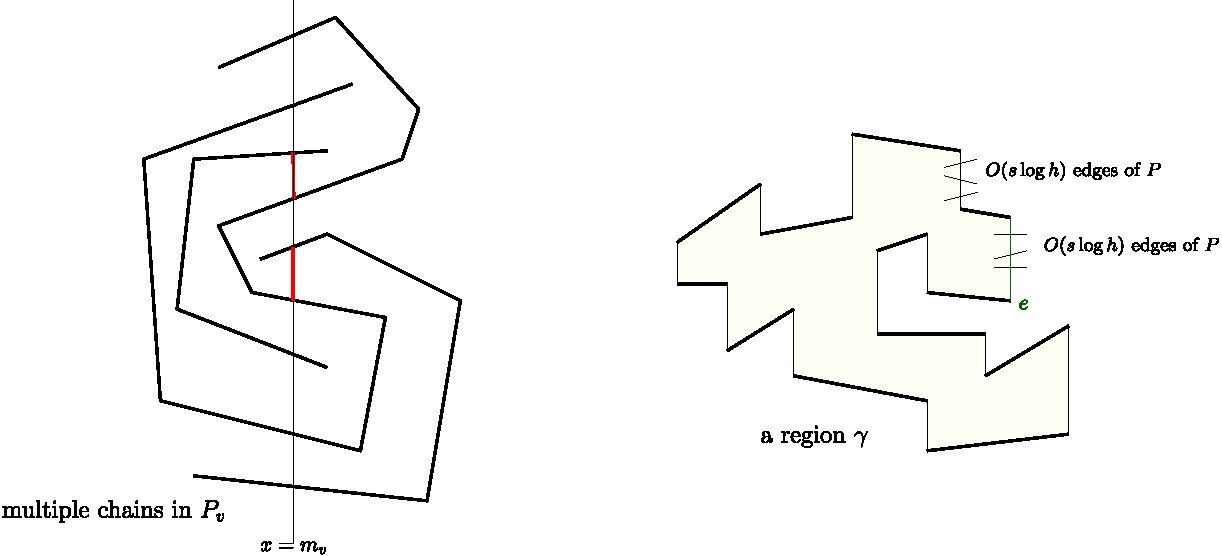
\includegraphics[width=0.7\linewidth,height=0.38\textheight,keepaspectratio]{fig_jordan_sort.pdf2svg.pdf}\end{center}
 Figure 2: (Left) In Step 1b, we can join multiple chains in $P_{v}$ intersecting a vertical line $x=m_{v}$ into a single component, for example, by adding the red vertical segments shown. (Right) In Step 4, we find the $O(s\log h)$ edges of $P$ intersecting each vertical side $e$ of a region $\gamma$; the non-vertical sides are parts of edges of $R$. Each region $\gamma$ is the union of $O(t)$ trapezoids of $\textit{TD}(R)$, and the total number of sides over all regions $\gamma$ is $O(|R|/\sqrt{t})$.  
\item[]  3. 
Compute $\textit{TD}(R)$ in $O(|R|\log|R|)$ time, and compute a $t$-division of the dual of $\textit{TD}(R)$ in $O(|R|)$ time.
\par
\par
\item[]  4. 
For each region $\gamma$ in the $t$-division and each vertical side $e$ of the boundary $\partial\gamma$, compute all intersections of $e$ with $P$. Since the interior of $e$ does not intersect $R$, we know that $e$ has at most $O(s\log h)$ intersections with $P$ by property (${\dagger}$), and they can be found in $O((\log n+s)\log h)$ time. (See Figure 2 (right).) By summing over all $O(|R|/\sqrt{t})$ choices of $e$, there are at most $O((|R|/\sqrt{t})\cdot s\log h)$ such intersections in total and they can be found in $O((|R|/\sqrt{t})\cdot(\log n+s)\log h)$ time.
\par
\par
Cut the chains of $P$ at all these intersection points to obtain a new collection $P^{\prime}$ of polygonal chains. In order to cut, we may need to sort the intersections along each edge of $P$, but this costs at most a logarithmic factor per intersection, i.e., $O((|R|/\sqrt{t})\cdot s\log h\cdot\log n)$ in total. The number of vertices in $P^{\prime}$ is $n^{\prime}\leq n+O((|R|/\sqrt{t})\cdot s\log h)$, and the number of chains in $P^{\prime}$ is $h^{\prime}\leq h+O((|R|/\sqrt{t})\cdot s\log h)$.
\par
\par
\item[]  5. 
For each region $\gamma$ in the $t$-division, let $P^{\prime}_{\gamma}$ be the chains of $P^{\prime}$ inside $\gamma$, and compute $\textit{TD}(P^{\prime}_{\gamma})$ by applying Bar-Yehuda and Chazelle’s previous algorithms [3] in $O(n^{\prime}_{\gamma}+h^{\prime}_{\gamma}\log^{O(1)}h^{\prime}_{\gamma})$ time, where $n^{\prime}_{\gamma}$ and $h^{\prime}_{\gamma}$ are the number of vertices and chains in $P^{\prime}_{\gamma}$ respectively.\footnote{We could avoid Bar-Yehuda and Chazelle’s algorithm and use some slower algorithm running in $O(n^{\prime}_{\gamma}+(h^{\prime}_{\gamma})^{O(1)})$ time, if we bootstrap one more time. } Note that $\sum_{\gamma}n^{\prime}_{\gamma}=n^{\prime}$ and $\sum_{\gamma}h^{\prime}_{\gamma}=h^{\prime}$. Furthermore, $\max_{\gamma}h^{\prime}_{\gamma}\leq O(t\cdot s\log h)$ (since there are at most $O(t)$ sides in $\gamma$, and at most $O(t)$ start vertices of chains inside $\gamma$ due to those extra segments of zero length added to $R$).
\par
\par
Afterwards, we can piece together $\textit{TD}(P^{\prime}_{\gamma})$ (after clipping to $\gamma$) over all regions $\gamma$, to obtain $\textit{TD}(P)$ in $O(n^{\prime})$ additional time.
\par
\par
\end{enumerate}
\par
% END S3.SS0.SSS0.P0.SPx1.p2
% BEGIN S3.SS0.SSS0.P0.SPx1.p3
The total running time for Steps 0–1 is $O(n+h\log h)$. The running time for Step 3 is $O(|R|\log|R|)=O((n/\sqrt{s}+h)\log n)$ time, as $|R|=O(n/\sqrt{s}+h)$. The total running time for Steps 4–5 is at most $O(n+((|R|/\sqrt{t})\cdot s\log h\cdot\log n)+(h+(|R|/\sqrt{t})\cdot s\log h)%
\log^{O(1)}(t\cdot s\log h))$.
\par
\par
% END S3.SS0.SSS0.P0.SPx1.p3
% BEGIN S3.SS0.SSS0.P0.SPx1.p4
Setting $s=\log^{2}n$ and $t=\log^{8}n$ gives an overall time bound of $O(n+h\log n+h(\log\log n)^{O(1)})=O(n+h\log n)$, which is the same as $O(n+h\log h)$ (since the second term dominates only if $h\geq n/\log n$, but then $\log n=O(\log h)$). $\hfill\blacktriangleleft$
\par
\par
% END S3.SS0.SSS0.P0.SPx1.p4
% BEGIN S3.SS0.SSS0.P0.SPx1.p5
As a corollary, we can test whether a collection $P$ of $h$ polygonal chains has any intersection in $O(n+h\log h)$ deterministic time: simply run the above algorithm to attempt to compute $\textit{TD}(P)$, and run Chazelle’s linear-time algorithm [5] to check simplicity of the resulting (connected) diagram.
\par
\par
% END S3.SS0.SSS0.P0.SPx1.p5
% END S3.SS0.SSS0.P0.SPx1
% END S3
% BEGIN bib
\par\medskip\noindent\textbf{References}\par
\begin{enumerate}
\item[]  [1]  Nancy M. Amato, Michael T. Goodrich, and Edgar A. Ramos.  A randomized algorithm for triangulating a simple polygon in linear time.  Discret. Comput. Geom., 26(2):245–265, 2001.  doi:10.1007/S00454-001-0027-X.  
\item[]  [2]  Ivan J. Balaban.  An optimal algorithm for finding segments intersections.  In Proc. 11th Annual Symposium on Computational Geometry (SoCG), pages 211–219, 1995.  doi:10.1145/220279.220302.  
\item[]  [3]  Reuven Bar-Yehuda and Bernard Chazelle.  Triangulating disjoint Jordan chains.  Int. J. Comput. Geom. Appl., 4(4):475–481, 1994.  doi:10.1142/S0218195994000252.  
\item[]  [4]  Jon Louis Bentley and Thomas Ottmann.  Algorithms for reporting and counting geometric intersections.  IEEE Trans. Computers, 28(9):643–647, 1979.  doi:10.1109/TC.1979.1675432.  
\item[]  [5]  Bernard Chazelle.  Triangulating a simple polygon in linear time.  Discret. Comput. Geom., 6:485–524, 1991.  doi:10.1007/BF02574703.  
\item[]  [6]  Bernard Chazelle and Herbert Edelsbrunner.  An optimal algorithm for intersecting line segments in the plane.  J. ACM, 39(1):1–54, 1992.  doi:10.1145/147508.147511.  
\item[]  [7]  Danny Z. Chen and Haitao Wang.  A new algorithm for computing visibility graphs of polygonal obstacles in the plane.  J. Comput. Geom., 6(1):316–345, 2015.  doi:10.20382/JOCG.V6I1A14.  
\item[]  [8]  Kenneth L. Clarkson, Richard Cole, and Robert Endre Tarjan.  Randomized parallel algorithms for trapezoidal diagrams.  Int. J. Comput. Geom. Appl., 2(2):117–133, 1992.  doi:10.1142/S0218195992000081.  
\item[]  [9]  Kenneth L. Clarkson and Peter W. Shor.  Application of random sampling in computational geometry, II.  Discret. Comput. Geom., 4:387–421, 1989.  doi:10.1007/BF02187740.  
\item[]  [10]  Kenneth L. Clarkson, Robert Endre Tarjan, and Christopher J. Van Wyk.  A fast Las Vegas algorithm for triangulating a simple polygon.  Discret. Comput. Geom., 4:423–432, 1989.  doi:10.1007/BF02187741.  
\item[]  [11]  Mark de Berg, Otfried Cheong, Marc J. van Kreveld, and Mark H. Overmars.  Computational Geometry: Algorithms and Applications.  Springer, 3rd edition, 2008.  doi:10.1007/978-3-540-77974-2.  
\item[]  [12]  David Eppstein and Michael T. Goodrich.  Studying (non-planar) road networks through an algorithmic lens.  In Proc. 16th ACM International Symposium on Advances in Geographic Information Systems (GIS), page 16, 2008.  doi:10.1145/1463434.1463455.  
\item[]  [13]  David Eppstein, Michael T. Goodrich, and Darren Strash.  Linear-time algorithms for geometric graphs with sublinearly many edge crossings.  SIAM J. Comput., 39(8):3814–3829, 2010.  doi:10.1137/090759112.  
\item[]  [14]  Alain Fournier and Delfin Y. Montuno.  Triangulating simple polygons and equivalent problems.  ACM Trans. Graph., 3(2):153–174, 1984.  doi:10.1145/357337.357341.  
\item[]  [15]  Greg N. Frederickson.  Fast algorithms for shortest paths in planar graphs, with applications.  SIAM J. Comput., 16(6):1004–1022, 1987.  doi:10.1137/0216064.  
\item[]  [16]  Michael T. Goodrich.  Planar separators and parallel polygon triangulation.  J. Comput. Syst. Sci., 51(3):374–389, 1995.  doi:10.1006/JCSS.1995.1076.  
\item[]  [17]  David Haussler and Emo Welzl.  $\varepsilon$-nets and simplex range queries.  Discret. Comput. Geom., 2:127–151, 1987.  doi:10.1007/BF02187876.  
\item[]  [18]  Kurt Hoffman, Kurt Mehlhorn, Pierre Rosenstiehl, and Robert Endre Tarjan.  Sorting Jordan sequences in linear time using level-linked search trees.  Inf. Control., 68(1-3):170–184, 1986.  doi:10.1016/S0019-9958(86)80033-X.  
\item[]  [19]  Sanjiv Kapoor and S. N. Maheshwari.  Efficiently constructing the visibility graph of a simple polygon with obstacles.  SIAM J. Comput., 30(3):847–871, 2000.  doi:10.1137/S0097539795253591.  
\item[]  [20]  David G. Kirkpatrick, Maria M. Klawe, and Robert Endre Tarjan.  Polygon triangulation in $O(n\log\log n)$ time with simple data structures.  Discret. Comput. Geom., 7:329–346, 1992.  doi:10.1007/BF02187846.  
\item[]  [21]  Philip N. Klein, Shay Mozes, and Christian Sommer.  Structured recursive separator decompositions for planar graphs in linear time.  In Proc. 45th ACM Symposium on Theory of Computing (STOC), pages 505–514, 2013.  doi:10.1145/2488608.2488672.  
\item[]  [22]  Richard J. Lipton and Robert Endre Tarjan.  Applications of a planar separator theorem.  SIAM J. Comput., 9(3):615–627, 1980.  doi:10.1137/0209046.  
\item[]  [23]  Jirí Matoušek.  Derandomization in computational geometry.  In Jörg-Rüdiger Sack and Jorge Urrutia, editors, Handbook of Computational Geometry, pages 559–595. North Holland / Elsevier, 2000.  doi:10.1016/B978-044482537-7/50014-0.  
\item[]  [24]  Joseph S. B. Mitchell, Valentin Polishchuk, Mikko Sysikaski, and Haitao Wang.  An optimal algorithm for minimum-link rectilinear paths in triangulated rectilinear domains.  Algorithmica, 81(1):289–316, 2019.  doi:10.1007/S00453-018-0446-1.  
\item[]  [25]  Ketan Mulmuley.  A fast planar partition algorithm, I.  J. Symb. Comput., 10(3/4):253–280, 1990.  doi:10.1016/S0747-7171(08)80064-8.  
\item[]  [26]  Franco P. Preparata and Michael Ian Shamos.  Computational Geometry: An Introduction.  Springer, 1985.  doi:10.1007/978-1-4612-1098-6.  
\item[]  [27]  Raimund Seidel.  A simple and fast incremental randomized algorithm for computing trapezoidal decompositions and for triangulating polygons.  Comput. Geom., 1:51–64, 1991.  doi:10.1016/0925-7721(91)90012-4.  
\item[]  [28]  Robert Endre Tarjan and Christopher J. Van Wyk.  An $O(n\log\log n)$-time algorithm for triangulating a simple polygon.  SIAM J. Comput., 17(1):143–178, 1988.  doi:10.1137/0217010.  
\item[]  [29]  Haitao Wang.  A new algorithm for Euclidean shortest paths in the plane.  J. ACM, 70(2):11:1–11:62, 2023.  doi:10.1145/3580475.  
\end{enumerate}
% END bib

\end{document}
